In this part of the system the feature function for unary potential is expressed as a conditional probability of assigning a label to the current pixel given its features. With such setting, there can be many types of different features, which may also include contextual data. In the already mentioned article by Jamie Shotton, the key component of the unary potential is a texture-layout potential, which operated on a texton map, and not on the original image. Therefore, before the segmentation process can take place a classification into textons needs to be conducted. Then, each pixel is assigned to exactly one texton, which makes it possible to model the relations between textures of neighbouring pixels. However, the dataset generated for the experiments described in this chapter do not contain any texture information and the only difference between objects is their colours and shapes. Hence, instead of performing a process of textonisation, colour quantisation was introduced. Then, each assignment of the pixel to a given colour from the reduced colour palette simulates the assignment to a single texton. As images from the generated dataset contain three main colours, after the quantisation process tricoloured images are obtained, as presented in figure \ref{fig:nonlinear_quantisation}.
\begin{figure}[ht]
    \centering
    \begin{tabular}{ccc}
        \fcolorbox{black}{white}{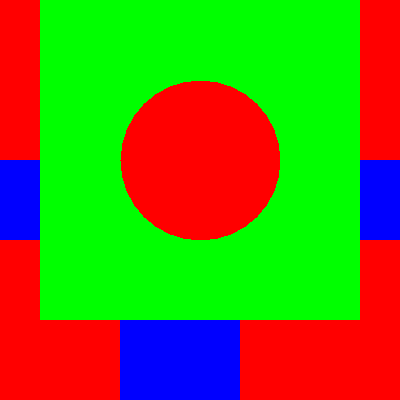
\includegraphics[width = 0.28\textwidth]{nonlinear_intro/circle_quant.png}} &
        \fcolorbox{black}{white}{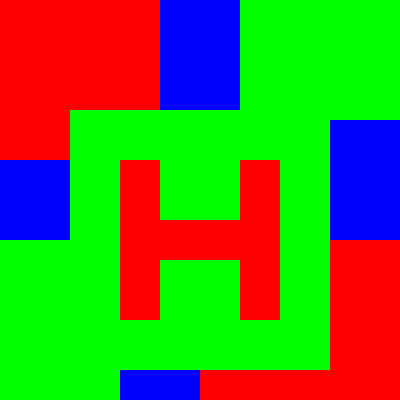
\includegraphics[width = 0.28\textwidth]{nonlinear_intro/letter_h_quant.png}} &
        \fcolorbox{black}{white}{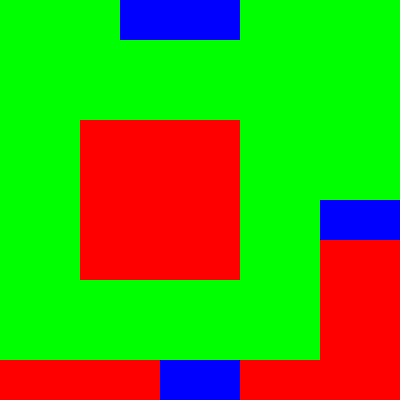
\includegraphics[width = 0.28\textwidth]{nonlinear_intro/square_quant.png}} 
    \end{tabular}
    \caption{Sample images after the process of colour quantisation.}
    \label{fig:nonlinear_quantisation}
\end{figure}
Having the dataset transformed into colour maps there is a need to extract features that are going to be used to compute the aimed conditional probability. For the task of shape differentiation two types of features were introduced and both of them include contextual data. 

The very first step that is needed obtain such features is to define a boundary of influence for a given superpixel. It was achieved by creating a regular grid of points around the centre of mass of the chosen superpixel. The distance between grid points is defined as the mean distance between neighbouring superpixel centres and the size of a created grid is a hyperparameter that should be fixed before feature extraction takes place. Then, each point in a grid represent a neighbour, which have an influence on a given superpixel.
\begin{figure}[ht]
    \centering
    \begin{subfigure}[h]{0.40\textwidth}
        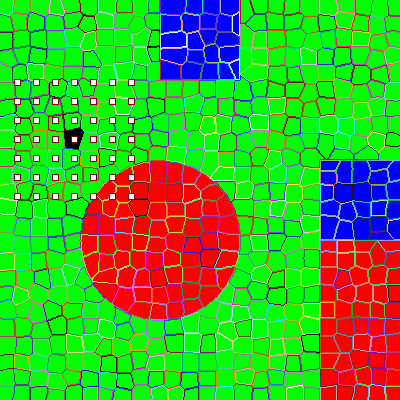
\includegraphics[width=\textwidth]{nonlinear_intro/grid_3.png}
        \caption{grid $7 \times 7$}
        \label{fig:grid_7_7}
      \end{subfigure}
    \begin{subfigure}[h]{0.40\textwidth}
        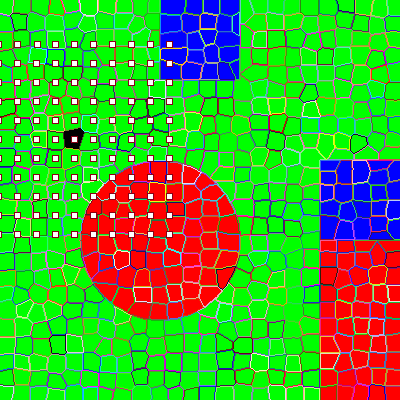
\includegraphics[width=\textwidth]{nonlinear_intro/grid_5.png}
        \caption{grid $11 \times 11$}
      \end{subfigure}
    \caption{Sample grid defining region of influence for a given superpixel.}
    \label{fig:nonlinear_grid}
\end{figure}
 Figure \ref{fig:nonlinear_grid} presents two grids, a $7 \times 7$ and $11 \times 11$ grid, that were created for the same sample superpixel in the same image which is marked with a black colour.

Having defined which superpixels have an influence on a superpixel under consideration it is possible to define its feature vector. The first type of features that was used in the described system are colours of the superpixels from the grid. Those features are discrete, as after the process of colour quantisation only three values are available: red, green, and blue. Hence, taking for example a superpixel from a grid depicted in figure \ref{fig:grid_7_7}, the contextual colour feature can be expressed as a vector of 49 values, each being a colour of one superpixel. Figure \ref{fig:grid_colour} depicts a visual representation of values from this vector with each feature being shown as a separate coloured box. The feature of a colour of the superpixel under consideration was marked with a pink border.
\begin{figure}[ht]
    \centering
    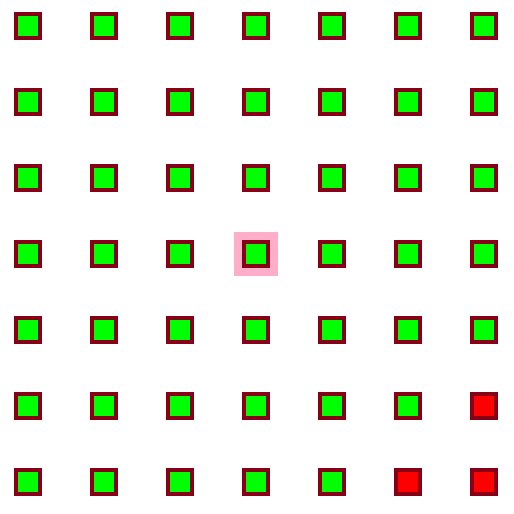
\includegraphics[width=0.5\textwidth]{nonlinear_intro/grid_colour.png}
    \caption{Neighbour colour features for a sample superpixel}
    \label{fig:grid_colour}
\end{figure}

The second type of features that were used in the system are also based on the described grid. However, instead of taking the colour of a superpixel in which a grid point lies, the colours of this superpixel neighbours are taken into consideration. For every superpixel from the grid, the percentage of red, green and blue colour in its neighbours is computed. Hence, for a grid $7 \times 7$ there are 49 triplets, which gives all together additional 147 features. Figure \ref{fig:grid_colour_neighbour} serves as an example on how those features are calculated.
\begin{figure}[ht]
    \centering
    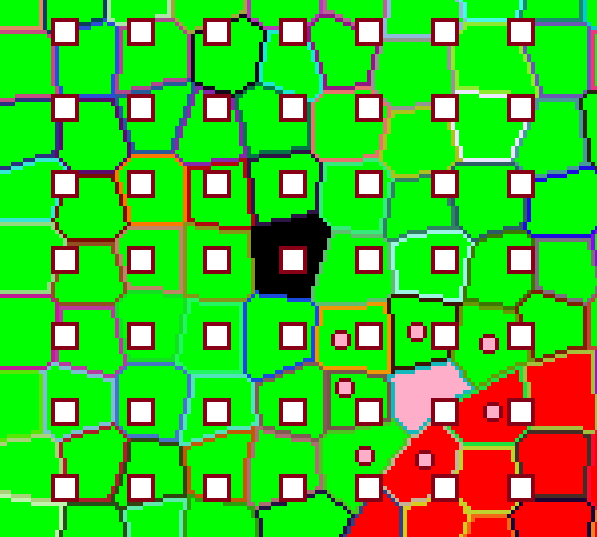
\includegraphics[width=0.5\textwidth]{nonlinear_intro/grid_neighbours.png}
    \caption{Neighbour colour percentage features for a sample superpixel}
    \label{fig:grid_colour_neighbour}
\end{figure}
In this image, values of \nth{121}, \nth{122} and \nth{123} features are to be computed, which are the percentage of red, green and blue neighbours for a superpixel that is marked in pink. This superpixel has seven closest neighbours, each marked with a pink circle, out of which five are green, two are red, and none are blue. Therefore, value of the \nth{121} feature will be equal to around 0.29, \nth{121} feature will have a value of 0.71, and for \nth{123} feature it will be 0. In such a way, every feature for every superpixel is computed. Similarly, as in case of the previous type of features, also a visual representation of computed features might be useful especially when comparing two different superpixels. Figure \ref{fig:grid_colour_neighbour_percentage} depicts such a representation. 
\begin{figure}[ht]
    \centering
    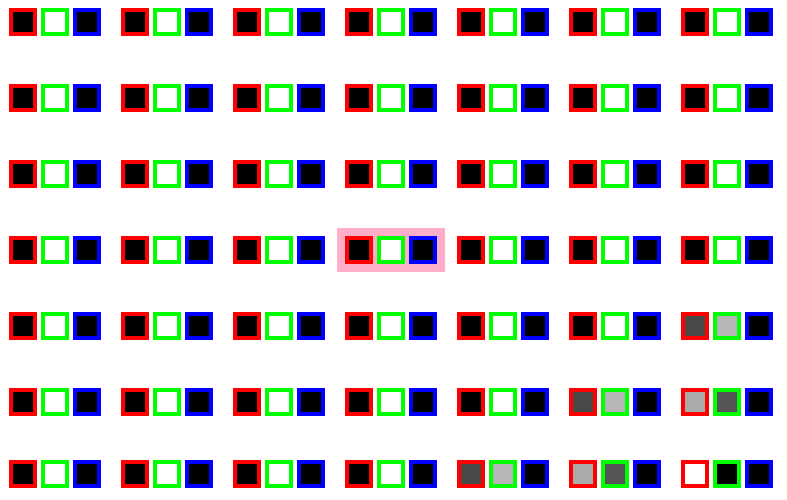
\includegraphics[width=\textwidth]{nonlinear_intro/grid_colour_percentage.png}
    \caption{Neighbour colour percentage features for a sample superpixel}
    \label{fig:grid_colour_neighbour_percentage}
\end{figure}
For each superpixel, three boxes are shown, one per each of the available colours, with a border representing this colour. The percentage of red, green or blue neighbours is expressed as a number between 0 and 1, which is then is multiplied by 255. The inner colour of every box is exactly this value. It can be easily seen, where there is a boundary between a green and a red region, as the features expressing percentage of green neighbours are gradually changing their colour from all white, meaning 100\% of green neighbours to all black meaning 0\% and conversely a feature for red percentage goes through through greyscale colours from black to white. Yet again, features of the superpixels that is under consideration are marked with a pink border.

Presented example was based on the grid $7 \times 7$ in which the percentage of neighbours of the given colour was computed on the adjacent superpixels only. However, sometimes it might be beneficial to include a larger neighbourhood. Then, instead of taking only adjacent superpixels, also neighbours of those superpixels could be taken into account. The size of this neighbourhood may have a large influence on the results, especially on the borders between two regions. With larger neighbourhood, even if a superpixel has only one neighbour of a different class, this neighbour may be mostly surrounded by superpixels with the same class, and therefore the total percentage of this class may rise. The neighbourhood size is yet another hyperparameter that should be fixed before feature extraction takes place.

With such definition of features, each superpixel can be defined in terms of a feature vector containing 196 elements. However, not all features but only a set of meaningful ones was used to compute a probability of a label conditioned on image features. A detailed description how this set was obtained will be presented in sections \textit{ \ref{sec:feature_selection_noise_free}} and \textit{\ref{sec:feature_selection_noise}: \nameref{sec:feature_selection_noise_free}}. Having a optimal feature vector constructed it is possible to express unary potential as a negative log-likelihood of a superpixel label given its features as in equation \ref{eq:nonlinear_unary_potential}. 
\begin{equation}
    \label{eq:nonlinear_unary_potential}
    \varphi(x_i,y_i) = -\log p(y_i|f_i)
\end{equation}
In order to compute a probability of a label conditioned on superpixel features it is necessary to know what is the probability distribution of all labels, and all available features. Estimation of this distribution is made only once, just after the stage of preprocessing, which divides images into superpixels. 